\documentclass[]{article}
\usepackage{lmodern}
\usepackage{amssymb,amsmath}
\usepackage{ifxetex,ifluatex}
\usepackage{fixltx2e} % provides \textsubscript
\ifnum 0\ifxetex 1\fi\ifluatex 1\fi=0 % if pdftex
  \usepackage[T1]{fontenc}
  \usepackage[utf8]{inputenc}
\else % if luatex or xelatex
  \ifxetex
    \usepackage{mathspec}
  \else
    \usepackage{fontspec}
  \fi
  \defaultfontfeatures{Ligatures=TeX,Scale=MatchLowercase}
\fi
% use upquote if available, for straight quotes in verbatim environments
\IfFileExists{upquote.sty}{\usepackage{upquote}}{}
% use microtype if available
\IfFileExists{microtype.sty}{%
\usepackage{microtype}
\UseMicrotypeSet[protrusion]{basicmath} % disable protrusion for tt fonts
}{}
\usepackage[margin=1in]{geometry}
\usepackage{hyperref}
\hypersetup{unicode=true,
            pdftitle={Solo 2: Discrete Choice Experiment},
            pdfauthor={Darryl Buswell},
            pdfborder={0 0 0},
            breaklinks=true}
\urlstyle{same}  % don't use monospace font for urls
\usepackage{longtable,booktabs}
\usepackage{graphicx,grffile}
\makeatletter
\def\maxwidth{\ifdim\Gin@nat@width>\linewidth\linewidth\else\Gin@nat@width\fi}
\def\maxheight{\ifdim\Gin@nat@height>\textheight\textheight\else\Gin@nat@height\fi}
\makeatother
% Scale images if necessary, so that they will not overflow the page
% margins by default, and it is still possible to overwrite the defaults
% using explicit options in \includegraphics[width, height, ...]{}
\setkeys{Gin}{width=\maxwidth,height=\maxheight}
\IfFileExists{parskip.sty}{%
\usepackage{parskip}
}{% else
\setlength{\parindent}{0pt}
\setlength{\parskip}{6pt plus 2pt minus 1pt}
}
\setlength{\emergencystretch}{3em}  % prevent overfull lines
\providecommand{\tightlist}{%
  \setlength{\itemsep}{0pt}\setlength{\parskip}{0pt}}
\setcounter{secnumdepth}{0}
% Redefines (sub)paragraphs to behave more like sections
\ifx\paragraph\undefined\else
\let\oldparagraph\paragraph
\renewcommand{\paragraph}[1]{\oldparagraph{#1}\mbox{}}
\fi
\ifx\subparagraph\undefined\else
\let\oldsubparagraph\subparagraph
\renewcommand{\subparagraph}[1]{\oldsubparagraph{#1}\mbox{}}
\fi

%%% Use protect on footnotes to avoid problems with footnotes in titles
\let\rmarkdownfootnote\footnote%
\def\footnote{\protect\rmarkdownfootnote}

%%% Change title format to be more compact
\usepackage{titling}

% Create subtitle command for use in maketitle
\newcommand{\subtitle}[1]{
  \posttitle{
    \begin{center}\large#1\end{center}
    }
}

\setlength{\droptitle}{-2em}
  \title{Solo 2: Discrete Choice Experiment}
  \pretitle{\vspace{\droptitle}\centering\huge}
  \posttitle{\par}
\subtitle{MSPA PREDICT 450-DL-55 LEC}
  \author{Darryl Buswell}
  \preauthor{\centering\large\emph}
  \postauthor{\par}
  \date{}
  \predate{}\postdate{}

\begin{document}
\maketitle

\section{1 Introduction}\label{introduction}

This document presents the results of the second assignment for the
Masters of Science in Predictive Analytics course: PREDICT 450. This
assessment required the student to estimate consumer preference shares
over choice scenarios for attributes of computer tablets, with the
intention of being used by an electronics manufacturer who is looking to
enter the tablet market.

For this assessment, the electronics manufacturer (Starful Technologies
Company (STC)) provided four different choice scenarios for preference
share modelling which were based on a wider set of survey results
administered by NeverMind Marketing Insights. The survey results were
used in order to fit two Hierarchical Bayes (HB) Multinomial Logit (MNL)
models for preference shares. These models were to allow for the
measurement of price sensitivity of respondent choices which are brand
specific and also for examination of the possible effects of prior STC
product ownership and respondent gender on the attributes' contributions
to preferences.

\section{2 Data}\label{data}

For this assessment, we were provided with consumer survey data from 360
respondents. The survey was designed and administered by STC and
NeverMind and included questions focused on consumer interest,
demographics and choice sets. The full set of survey questions included:

\begin{itemize}
\tightlist
\item
  STCOwner: Previous owner of an STC product?
\item
  36 choice set questions
\item
  Interest questions:

  \begin{itemize}
  \tightlist
  \item
    Purchasing a new tablet?
  \item
    Purchasing a new smart phone?
  \item
    Using cloud storage for storing personal digital content?
  \item
    Taking an online course to improve relevant skills?
  \end{itemize}
\item
  Gen: Gender of respondent
\item
  Age: Age of respondent
\end{itemize}

The 36 choice set questions were build from the following five
attributes:

\begin{itemize}
\tightlist
\item
  Brand: 4 levels: STC, Somesong, Pear, Gaggle (level codes: 0,1,2,3)
\item
  Price: 3 levels: \$199, \$299, \$399 (level codes: 0,1,2)
\item
  Screen: 3 levels: 5 inch, 7 inch, 10 inch (level codes: 0,1,2)
\item
  RAM: 3 levels: 8 Gb, 16 Gb, 32 Gb (Gb = ``gigabytes'') (level codes:
  0,1,2)
\item
  Processor: 3 levels: 1.5 GHz, 2 GHz, 2.5 GHz (GHz = ``gigahertz'')
  (level codes: 0,1,2)
\end{itemize}

Each of the 36 choice set questions had three alternatives with each
alternative representing a specific combination of the above attribute
levels (108 possibilities). Each consumer was to rank the three
alternatives presented for each choice set with a score from one to
three.

We were also provided with two additional datasets. The first is a
dataframe of the 108 possible combinations of alternatives for the 36
choice set questions above. The second is a dataframe of 12 alternatives
based on the choice sets of four additional respondents. The first of
these datasets is to be used to form the predictor variable set for
model estimation while the second is to be used for subsequent
preference share modelling.

\section{3 Data Pre-processing}\label{data-pre-processing}

A number of data pre-process routines were conducted in order to
manipulate the data into a format which can easily allow fitting of the
MNL regression models. These routines and their outputs are explained in
their order of execution below:

\begin{enumerate}
\def\labelenumi{\arabic{enumi})}
\tightlist
\item
  Effects matrix: Generate a matrix which includes an effects coded
  version of the 108 possible combinations of attributes from the
  original dataset.
\item
  Brands matrix: Extract the coded levels associated with brand from the
  `effects matrix'.
\item
  Price vector: Create a price vector of the difference between the
  price associated with each attribute combination and the mean price of
  all possible attribute combinations.
\item
  Brand by price matrix: Multiply the `brands matrix' by the `price
  vector' in order to create a matrix of interactions between brand and
  price.
\item
  X-matrix: Merge the `effects matrix' and the `brands by price matrix'
  to create a `X-matrix' of predictor variables for the modelling phase.
\item
  y-data: Extract each respondents selection to the 36 choice set
  questions from the original dataset.
\item
  List of y by X-matrix: Create a list of combinations of each
  respondents selection to the 36 choice questions (y-matrix) and the
  matrix of predictor variables (X-matrix).
\end{enumerate}

\section{4 Model Estimation}\label{model-estimation}

For this assessment, we fit two HB MNL models for preference shares
using the R function rhierMnIDP from the bayesm R package. One model
includes a covariate indicating previous ownership of a STC product and
a covariate for respondent gender, while the other model excludes these
covariates. Both models were estimated using Markov Chain Monte Carlo
(MCMC) simulation, for which we elected to include 30,000 iterations and
retain every 10th sample.

\subsection{4.1 Model 1}\label{model-1}

The first model (Model 1), includes the choice set responses for all 360
respondents (y-data) along with predictor variables (X-matrix). The
functional form of the MNL likelihood model used for Model 1 can be
shown as:

\(y_{ijk} = X_{ijk} \cdot \beta_{i} + e_{ijk}\)

where:

\(\beta_i\) \textasciitilde{}
\(MVN\left(\overline{\beta },V_{\beta}\right)\)

There are a number of statistical methods available to assess the
overall model fit, including Mean Squared Error (MSE), Mean Absolute
Error (MAE), likelihood measures (such as LL, RLH, and pseudo
R-squared), Bayes factor, and posterior predictive checks. To calculate
these statistical measures one would need to first find the posterior
means for each beta of each respondent. Next, a matrix would be derived
from multiplying the original X-matrix by the posterior means, which
would then be exponentiated and divided by the row sums of exponentiated
betas. For this assessment however, we elect to instead conduct a simple
`sniff test', by first ensuring we have included enough iterations for
proper `burn-in' of coefficients, and then to assess the beta means
directly to determine whether each seem logical.

\newpage

The betadraws recorded over the MCMC simulation for Model 1 are shown in
the figure below.

\paragraph{Figure 4.1.1 Model 1
Betadraw}\label{figure-4.1.1-model-1-betadraw}

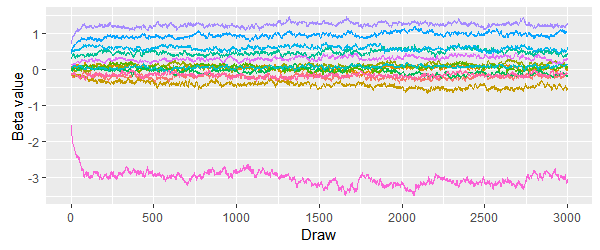
\includegraphics{images/model1_betadraw.png}

Likewise, the Log Likelihood values recorded over the MCMC simulation
for Model 1 are shown below.

\paragraph{Figure 4.1.2 Model 1 Log
Likelihood}\label{figure-4.1.2-model-1-log-likelihood}

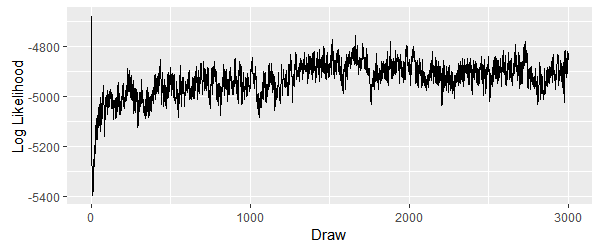
\includegraphics{images/model1_loglike.png}

We can see that the beta and likelihood value tend to level out at
around 2,000 iterations, suggesting that we have included more than
enough iterations to achieve a proper burn-in.

The table below shows the beta means for each attribute.

\newpage

\paragraph{Table 4.1.1 Model 1 Beta
Means}\label{table-4.1.1-model-1-beta-means}

\begin{longtable}[]{@{}llr@{}}
\toprule
& Attribute & Beta mean\tabularnewline
\midrule
\endhead
screen\_1 & 7 inch Screen & -0.181\tabularnewline
screen\_2 & 10 inch Screen & 0.486\tabularnewline
RAM\_1 & 16Gb RAM & 0.080\tabularnewline
RAM\_2 & 32Gb RAM & 0.616\tabularnewline
processor\_1 & 2GHz Processor & 0.939\tabularnewline
processor\_2 & 2.5Ghz Processor & 1.262\tabularnewline
price\_1 & \$299 & 0.311\tabularnewline
price\_2 & \$399 & -2.907\tabularnewline
brand\_1 & Somesong Brand & -0.111\tabularnewline
brand\_2 & Pear Brand & 0.046\tabularnewline
brand\_3 & Gaggle Brand & -0.393\tabularnewline
brand\_1\_by\_Price & Somesong Brand by Price & 0.126\tabularnewline
brand\_2\_by\_Price & Pear Brand by Price & 0.047\tabularnewline
brand\_3\_by\_Price & Gaggle Brand by Price & 0.008\tabularnewline
\bottomrule
\end{longtable}

Since we generated an effects coded version of the attribute data as
part of the pre-processing routine, we do not directly estimate beta
mean values for the reference level of each attribute (level code: 0).
We instead estimate the beta mean for the reference level by solving the
sum of beta means for all levels of that attribute for zero. In this
case, solving for zero is appropriate as our specification lacks an
intercept term. An example would be for the RAM attribute, where we have
a beta mean estimate of 0.080 and 0.616 for the second and third levels
of this attribute (level code 1: 16 Gb, level code 2: 32 Gb). In this
case, the beta estimate for the first level of the RAM attribute (level
code 0: 8gb) would be equal to 0.304 (1-0.616-0.080).

From an assessment of the beta means for each attribute, we note that
respondents seem to have a preference for tablets with a 10 inch screen,
32 Gb of RAM, 2.5 GHz processor speed, at a \$199 price point, and of
the STC brand. The attribute preferences for screen size, RAM and
processor speed seem reasonable, noting that greater levels for these
attributes coincide with values which can be seen to provide `functional
value'. i.e.~a greater amount of RAM is seen to provide more value than
less RAM. Likewise the preference for a lower price point seems
reasonable. We have little justification for the STC brand preference,
although we do note that the small magnitude of coefficient for each
brand attribute.

Finally, there does not seem to be a great deal of variation in mean
betas for our brand by price interaction terms and likewise the beta
means for each are close to zero. This would suggest little price
sensitivity between brands. However, to further assess whether price
sensitivity does in fact vary by brand, we can derive the distribution
of beta estimates for the final 300 draws of each of the brand by price
attribute, and then determined the number of draws which fall outside of
the 5th and 95th percentiles of each distribution. The results can be
seen in the table below.

\begin{longtable}[]{@{}lr@{}}
\toprule
& \% of draws outside 5th/95th percentiles\tabularnewline
\midrule
\endhead
brand\_1\_by\_Price & 2.3\%\tabularnewline
brand\_2\_by\_Price & 1.3\%\tabularnewline
brand\_3\_by\_Price & 0.1\%\tabularnewline
\bottomrule
\end{longtable}

We note that each brand has only a small amount of draws which fall
beyond the 5th and 95th percentiles of each distribution.

\subsection{4.2 Model 2}\label{model-2}

The second model (Model 2), includes the choice set responses for all
360 respondents (y-data) along with predictor variables (X-matrix), but
also includes additional covariates of responses to the survey questions
``STCOwner'' and ``Gender''. We can then express the beta's as dependent
variables of the predictors (covariates):

\(\beta_{i} = \psi \cdot Z_{i} + u_{i}\)

where:

\(u_{i}\) \textasciitilde{} \(MVN\left(0,V_{u}\right)\)

As noted previously, there are a number of statistical methods available
to assess the overall model fit. For this assessment however, we again
elect to instead conduct a simple `sniff test'.

The betadraws recorded over the MCMC simulation for Model 2 are shown in
the figure below.

\paragraph{Figure 4.2.1 Model 2
Betadraw}\label{figure-4.2.1-model-2-betadraw}

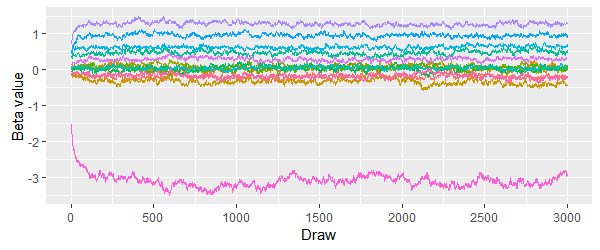
\includegraphics{images/model2_betadraw.png}

Likewise, the Log Likelihood values recorded over the MCMC simulation
for Model 2 are shown below.

\paragraph{Figure 4.2.2 Model 2 Log
Likelihood}\label{figure-4.2.2-model-2-log-likelihood}

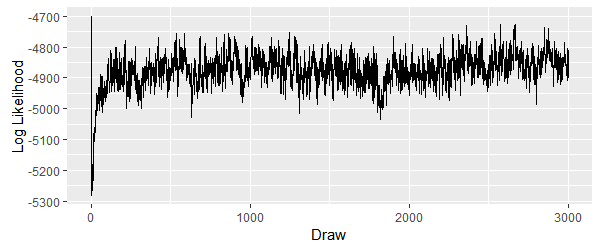
\includegraphics{images/model2_loglike.png}

We can see that the beta and likelihood value tend to level out at
around 1,000 iterations, suggesting that we have included more than
enough iterations.

The table below shows the beta means and delta means for each attribute.

\paragraph{Table 4.2.1 Model 2 Beta
Means}\label{table-4.2.1-model-2-beta-means}

\begin{longtable}[]{@{}llrrr@{}}
\toprule
& Attribute & Beta mean & STCOwner delta mean & Gender delta
mean\tabularnewline
\midrule
\endhead
screen\_1 & 7 inch Screen & -0.181 & 0.021 & -0.112\tabularnewline
screen\_2 & 10 inch Screen & 0.486 & -0.320 & -0.085\tabularnewline
RAM\_1 & 16Gb RAM & 0.080 & -0.141 & -0.076\tabularnewline
RAM\_2 & 32Gb RAM & 0.616 & -0.191 & -0.143\tabularnewline
processor\_1 & 2GHz Processor & 0.939 & 0.055 & -0.118\tabularnewline
processor\_2 & 2.5Ghz Processor & 1.262 & 0.751 & -0.206\tabularnewline
price\_1 & \$299 & 0.311 & 0.026 & -0.120\tabularnewline
price\_2 & \$399 & -2.907 & 0.442 & 0.160\tabularnewline
brand\_1 & Somesong Brand & -0.111 & -0.458 & 0.076\tabularnewline
brand\_2 & Pear Brand & 0.046 & 1.175 & -0.116\tabularnewline
brand\_3 & Gaggle Brand & -0.393 & 0.258 & -0.466\tabularnewline
brand\_1\_by\_Price & Somesong Brand by Price & 0.126 & 0.258 &
0.060\tabularnewline
brand\_2\_by\_Price & Pear Brand by Price & 0.047 & -0.136 &
0.186\tabularnewline
brand\_3\_by\_Price & Gaggle Brand by Price & 0.008 & -0.340 &
0.023\tabularnewline
\bottomrule
\end{longtable}

We can assess the delta means of both the `STCOwner' and `Gender'
covariates in order to determine whether prior ownership of an STC
product or gender has an impact on attribute preferences. For example,
the STCOwner delta means above suggest that those who have previously
owned an STC branded product can be seen to have a greater preference
for tablets with a 5 inch screen, 8 Gb of RAM, and 2.5 GHz processor
speed, at a \$399 price point. This result is at odds to those suggested
by the beta mean values. It is also surprising that those who previously
owned an STC branded product had a much greater preference for Pear
branded products. We can see a similar bias toward performance
attributes for males. That is, males can also be seen to have a greater
preference for tablets with a 5 inch screen and 8 Gb of RAM. But in this
case, males also have a greater preference for 1.5Ghz processor speed
and STC branded products.

\section{5 New Choice Scenario}\label{new-choice-scenario}

We can now use the estimated models to estimate preference shares for
the alternatives in each of the four additional scenarios. To do this,
we first create an X-matrix which includes an effects coded version of
the additional provided scenarios. We then calculate the posterior means
for each beta for each subject by using the betas from Model 1 and then
multiply this matrix by the transpose of the mean betas matrix. The
result is a matrix of the choice sets which can be converted to a matrix
of choice probabilities by exponentiating each row and dividing it by
its row sum.

We can use the choice probabilities in order to derive a set of
preference shares for each attribute. To do this, we must calculate the
conjoint part-worth utilities for each respondent. Quite simply,
part-worth utility can be found by dividing the sum of the number of
times an attribute was selected by the number of times the attribute was
available for selection. This ratio provides an indication of attribute
preference and can be used to measure the relative importance of
attributes. The table below shows the preference share for each
attribute over the four additional scenarios.

\newpage

\paragraph{Table 5.1 Preference
Shares}\label{table-5.1-preference-shares}

\begin{longtable}[]{@{}lrrr@{}}
\toprule
& share & pct.5\% & pct.95\%\tabularnewline
\midrule
\endhead
screen\_1 & 0.044 & 0.039 & 0.049\tabularnewline
screen\_2 & 0.254 & 0.243 & 0.265\tabularnewline
RAM\_1 & 0.059 & 0.053 & 0.065\tabularnewline
RAM\_2 & 0.044 & 0.037 & 0.052\tabularnewline
processor\_1 & 0.033 & 0.026 & 0.041\tabularnewline
processor\_2 & 0.021 & 0.016 & 0.027\tabularnewline
processor\_3 & 0.030 & 0.024 & 0.036\tabularnewline
price\_1 & 0.114 & 0.102 & 0.125\tabularnewline
price\_2 & 0.044 & 0.039 & 0.049\tabularnewline
brand\_1 & 0.254 & 0.243 & 0.265\tabularnewline
brand\_2 & 0.059 & 0.053 & 0.065\tabularnewline
brand\_3 & 0.044 & 0.037 & 0.052\tabularnewline
\bottomrule
\end{longtable}

We can see a relatively higher preference share for 10 inch Screen, at
the \$299 price point and of the Somesong Brand.

\section{6 Conclusion}\label{conclusion}

For this assessment, we fit two Hierarchical Bayes (HB) Multinomial
Logit (MNL) models in order to measure the price sensitivity of
respondent choices which are brand specific and to also examine the
possible effects of prior STC product ownership and respondent gender on
the attributes' contributions to preferences.

Firstly, an evaluation of the mean betas for brand by price interaction
terms of Model 1 showed us that there was little variation between mean
beta values and therefore little price sensitivity between brands. This
is a positive indicator for STC's decision to join the market. We also
evaluated the remaining mean betas of Model 1 and found that respondents
had a preference for tablets with a 10 inch screen, 32 Gb of RAM, 2.5
GHz processor speed, at a \$199 price point.

In terms of the effects of prior STC product ownership, we found that
the STCOwner delta means of Model 2 suggested that those who had
previously owned an STC product tend to have a preference for Pear
branded products. Clearly, STC would do well to target any advertising
campaign as part of their market entry against the Pear brand. The
Gender delta means of Model 2 also showed some interesting preferences
for male respondents, with their attribute preferences tending to favor
a smaller screen size, less RAM and slower processor speed.

It may be that STC would benefit from providing two product lines, the
first with a greater screen size, greater amount of RAM and faster
processor speed at a higher price point. The second with a smaller
screen size, less amount of RAM and slower processor speed at a lower
price point. The first of these products should be targeted towards
female consumers, while the second should be targeted towards male
consumers. However, the marketing campaign to introduce both of these
products should be targeted against the Pear brand.

\hypertarget{refs}{}


\end{document}
